\section{Resultados de la simulación}
\label{sec:resultados}

Cada misión libera a los insectos por un boquete de un colapso sintético de $8\times6$~m con
unos \areaLibre~m$^2$ de huecos; la persona está inmóvil, a un recorrido medio de
\distVictima~m de la entrada. Cada configuración se corrió \numCorridas{} veces en
\numMapas{} colapsos distintos: \numMisiones{} misiones de una hora. Con esa muestra, cada
porcentaje tiene un margen de unos $\pm5$ puntos (intervalo de 95~\%).

\subsection{Validación de la marcha}

Antes de comparar políticas se comprobó que el insecto simulado camina como el medido. En una
arena abierta de $1\times1$~m se midieron las mismas magnitudes que
reportan~\cite{dirafzoon2017,tranngoc2024}, primero sin estímulos y luego con comandos al azar.

\begin{table}[H]
\centering\footnotesize
\caption{Marcha simulada frente a la publicada.}
\label{tab:validacion}
\rowcolors{2}{SoftGray}{white}
\begin{tabularx}{0.86\textwidth}{@{}>{\raggedright\arraybackslash}X r r@{}}
\toprule
\rowcolor{TableHead} \textbf{Medida} & \textbf{Publicado} & \textbf{Simulación} \\
\midrule
Fracción del tiempo caminando, sin estímulos & $0.37\pm0.20$ & \valAndaNat \\
Pausa media, sin estímulos (s) & $36.8\pm24.1$ & \valPausaNat \\
Probabilidad de soltar la pared, sin estímulos & 0.005 & \valSalidaNat \\
Fracción del tiempo caminando, con comandos & 0.643 & \valAndaCom \\
Probabilidad de soltar la pared, con comandos & 0.052 & \valSalidaCom \\
Pausa media, con comandos (s) & 5.55 & \valPausaCom \\
\bottomrule
\end{tabularx}
\end{table}

Cinco de las seis medidas coinciden con lo publicado o caen dentro de su dispersión. La que no
coincide es la pausa con comandos: el insecto simulado descansa \valPausaCom~s y el real,
5.6~s. En ese punto el modelo es conservador, porque subestima cuánto acorta las pausas un
estímulo.

\subsection{Cuatro políticas con diez insectos}

Se comparan cuatro políticas. La \textbf{pasiva} solo detecta. La \textbf{antipausa} da un pulso de
avance cuando el insecto lleva 15~s quieto. La \textbf{estocástica} añade giros al azar. La
\textbf{guiada} es la del núcleo: además gira hacia el calor en cuanto la matriz ve dos píxeles.

\begin{figure}[H]
\centering
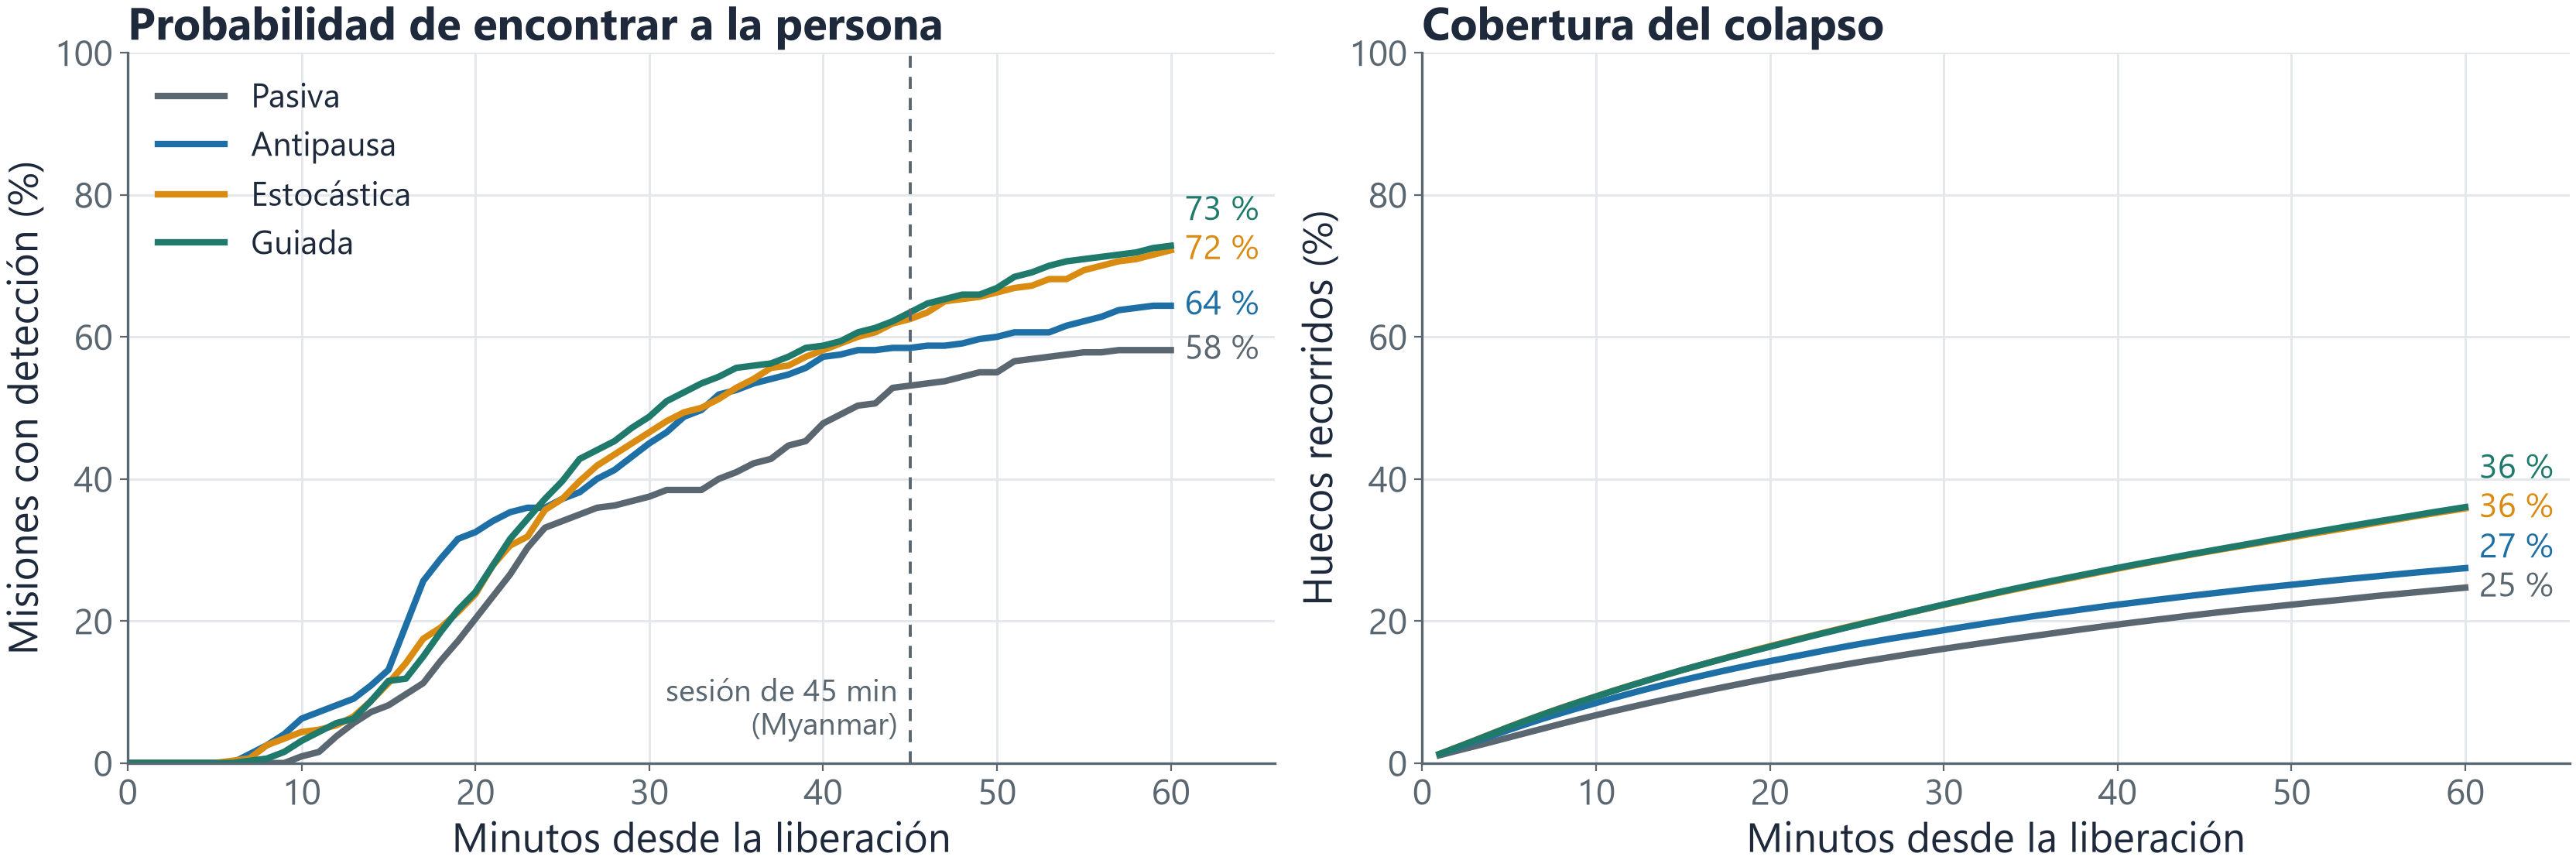
\includegraphics[width=\textwidth]{figs/resultados_politicas.png}
\caption{Diez insectos, \numMisiones{} misiones por política. Izquierda: fracción de misiones en que
algún insecto confirma a la persona. Derecha: fracción de los huecos por los que pasó al menos un insecto.}
\label{fig:politicas}
\end{figure}

\begin{table}[H]
\centering\footnotesize
\caption{Resultados por política con diez insectos. La mediana se calcula entre las misiones que detectan.}
\label{tab:politicas}
\rowcolors{2}{SoftGray}{white}
\begin{tabularx}{\textwidth}{@{}>{\bfseries\raggedright\arraybackslash}X r r r r r r r r@{}}
\toprule
\rowcolor{TableHead} & \multicolumn{4}{c}{\textbf{Detección acumulada (\%)}} & \textbf{Mediana} & \textbf{Cobertura} & \textbf{Estímulos por} & \textbf{Tiempo} \\
\rowcolor{TableHead} \textbf{Política} & 15 min & 30 min & 45 min & 60 min & (min) & (\%) & insecto y hora & caminando (\%) \\
\midrule
\tablaPoliticas
\bottomrule
\end{tabularx}
\end{table}

Sin estímulos, diez insectos encuentran a la persona en \pPasivaSesenta~\% de las misiones de
una hora. Reactivar al insecto cuando se queda quieto sube la cifra a \pAntipausaSesenta~\%;
añadir giros al azar, a \pEstocasticaSesenta~\%; y girar hacia el calor, a \pGuiadaSesenta~\%.
Tres lecturas:
\begin{itemize}
  \item \textbf{La ganancia viene de mantener al insecto en movimiento y despegarlo de las paredes.}
        Girar hacia el calor casi no añade, porque solo actúa dentro del alcance de la matriz.
  \item \textbf{En el primer cuarto de hora las políticas no se distinguen.} La diferencia aparece
        después de la media hora, cuando el insecto sin estímulos acumula pausas.
  \item \textbf{El costo es bajo:} unos \estGuiada{} estímulos por insecto y por hora, uno por minuto,
        siempre por debajo del presupuesto de doce acumulados.
\end{itemize}

\begin{figure}[H]
\centering
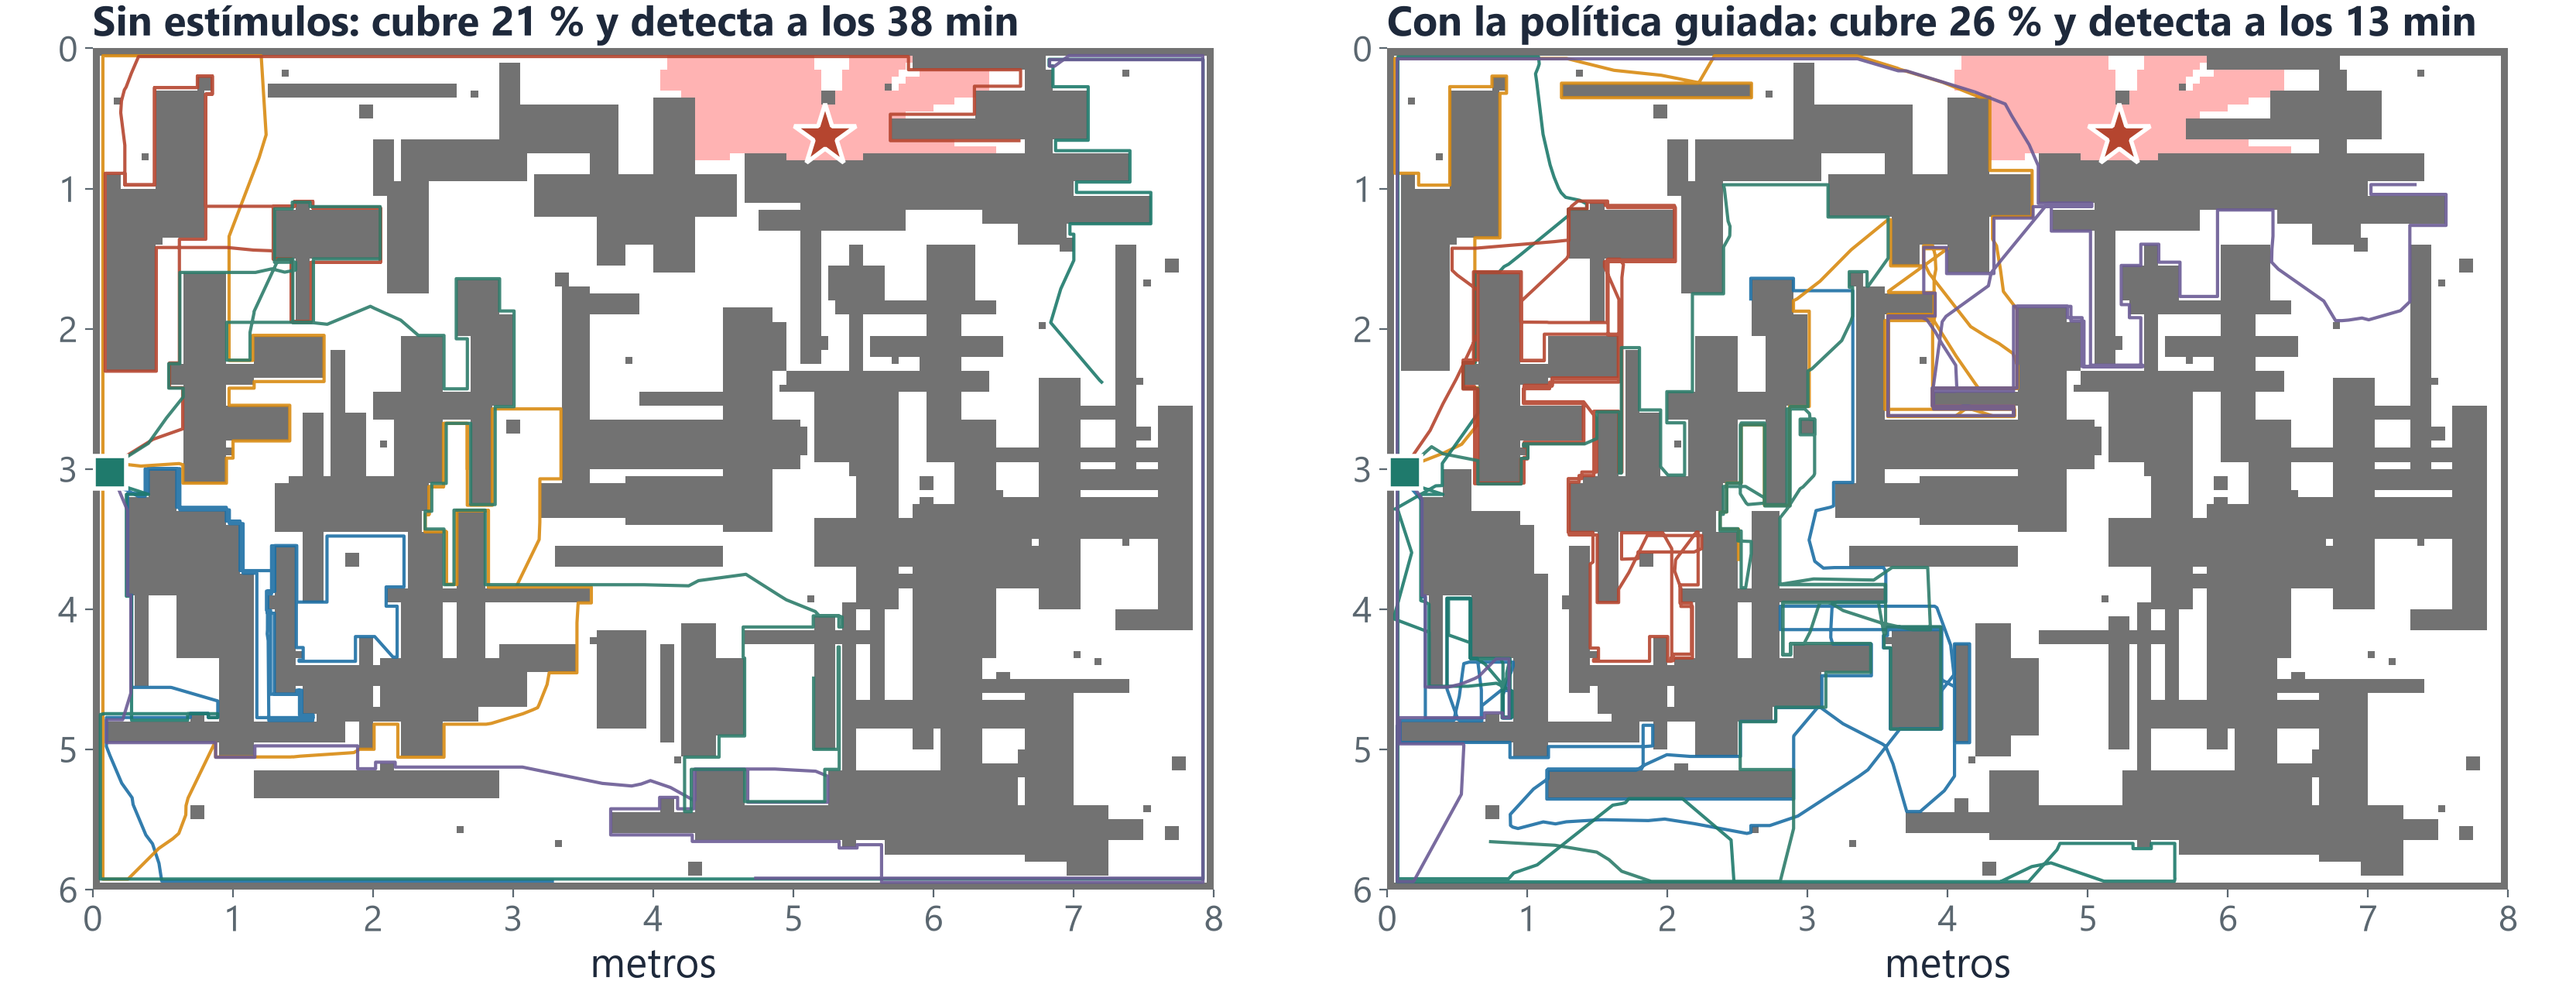
\includegraphics[width=\textwidth]{figs/mapa_trayectorias.png}
\caption{Una misión de ejemplo: seis insectos durante 45~min en el mismo colapso. Cuadro verde: entrada;
estrella: persona; zona sombreada: desde donde la matriz confirma. Una sola corrida no prueba nada; la
comparación válida es la de la figura~\ref{fig:politicas}.}
\label{fig:mapa}
\end{figure}

\subsection{El colapso pesa más que la política}

\begin{figure}[H]
\centering
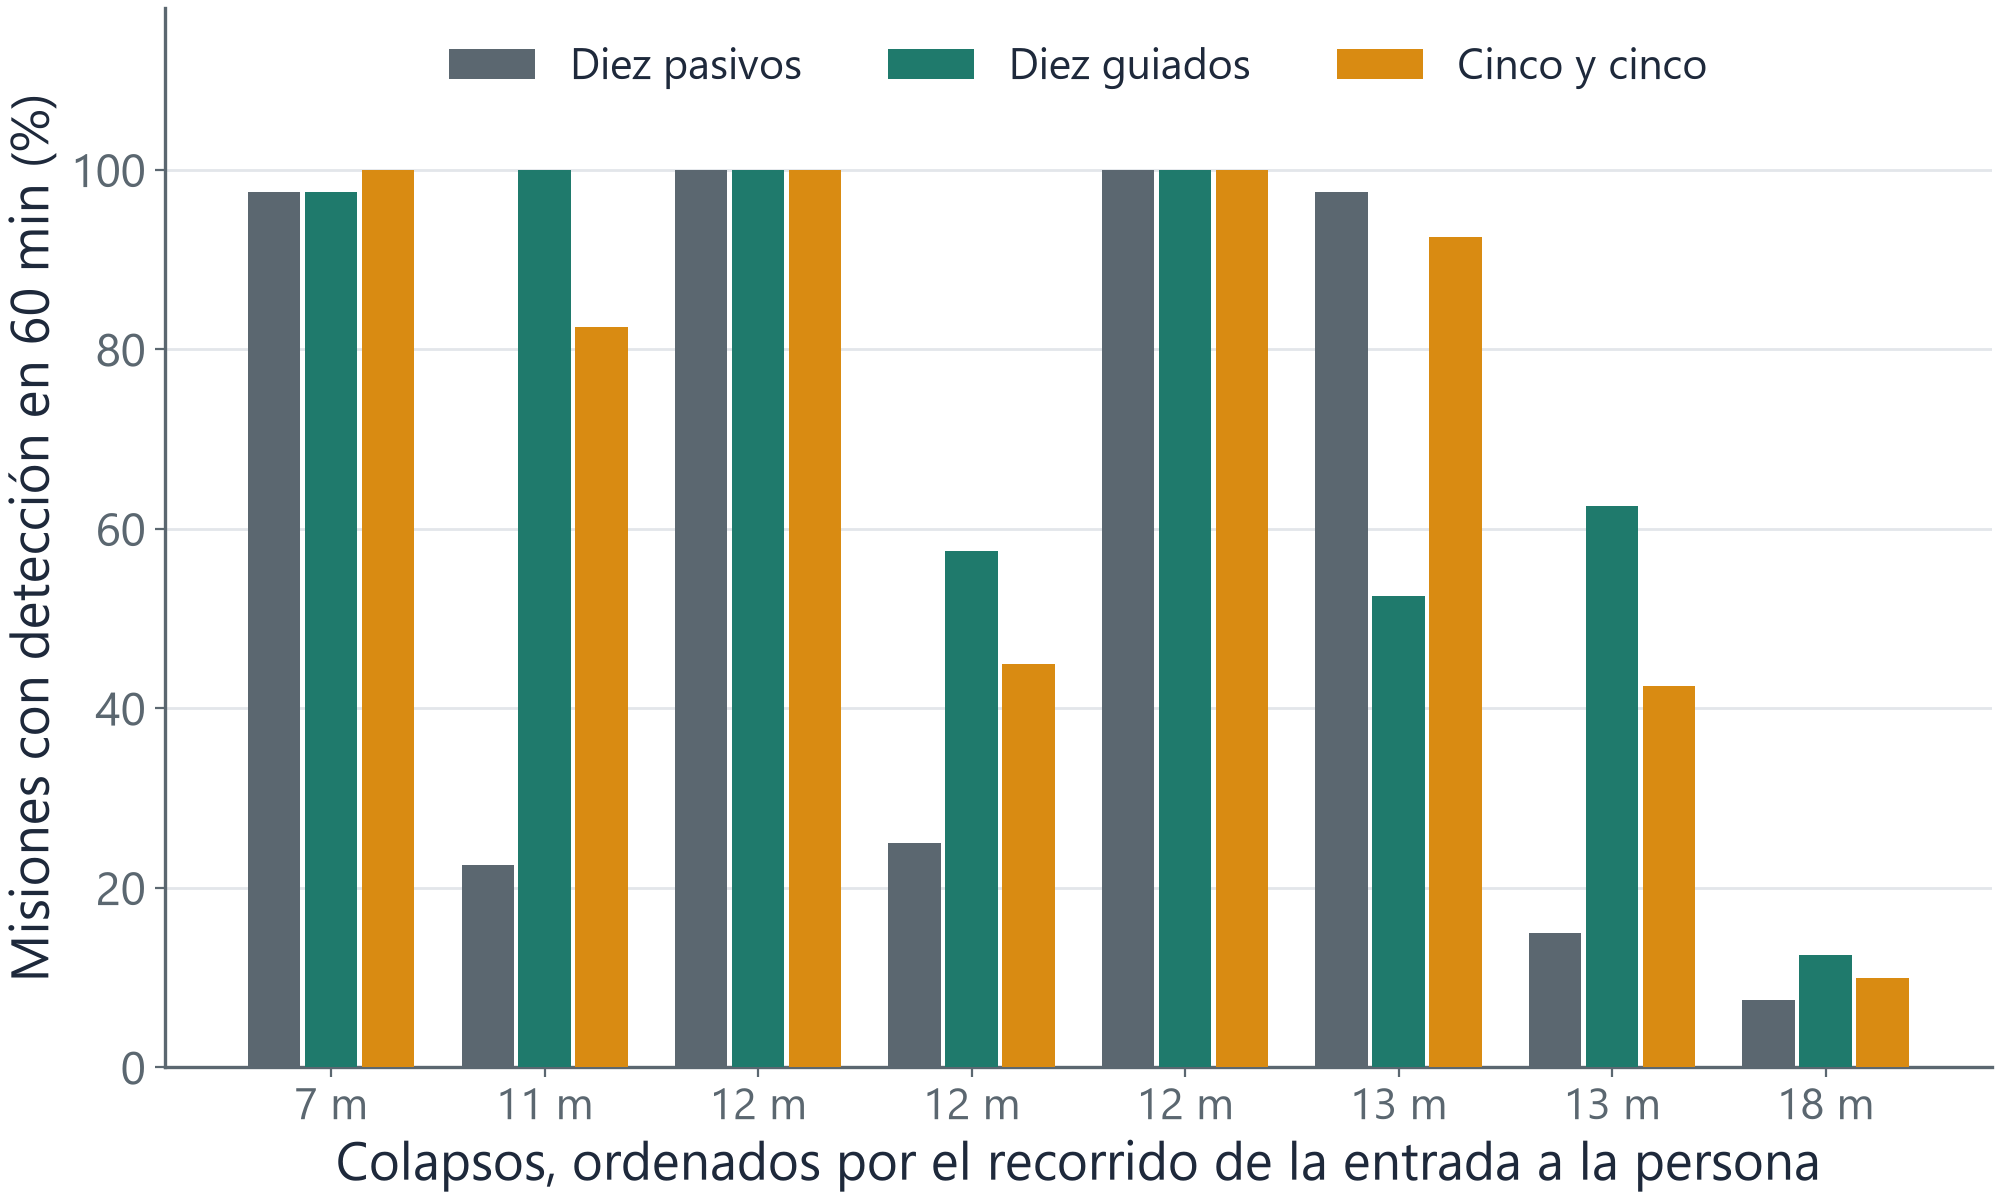
\includegraphics[width=0.7\textwidth]{figs/por_mapa.png}
\caption{Detección a 60~min en cada uno de los ocho colapsos, con diez insectos pasivos, diez guiados y
cinco de cada uno. Cuarenta misiones por barra.}
\label{fig:pormapa}
\end{figure}

El promedio esconde una dispersión grande. Según el colapso, la detección en una hora va de
\mapaMinPasiva{} a \mapaMaxPasiva~\% sin estímulos y de \mapaMinGuiada{} a \mapaMaxGuiada~\%
con la política guiada (figura~\ref{fig:pormapa}). La guiada gana por más de cinco puntos en
\mapasGanaGuiada{} de los \numMapas{} colapsos, empata en \mapasEmpate{} y pierde en
\mapasPierdeGuiada.

En los empates las dos políticas dan lo mismo porque la persona se encuentra de cualquier modo
o porque queda demasiado lejos para ambas. Donde la guiada gana, cambia el resultado por
completo: en el caso más claro, de \mapaMejorPasiva{} a \mapaMejorGuiada~\%. Y donde pierde,
pierde mucho: de \mapaPeorPasiva{} a \mapaPeorGuiada~\%. En ese colapso seguir la pared lleva
directo a la persona, y los giros al azar sacan al insecto de ese camino. El promedio de la
sección anterior, por lo tanto, no describe a ningún colapso en particular: en cada uno el
resultado es casi todo o casi nada, y lo decide la geometría.

\textbf{Un enjambre mixto cubre los dos casos.} Como desde afuera no se sabe qué tipo de colapso
se tiene, se probó liberar cinco insectos sin estímulos y cinco guiados. El promedio no cambia:
\mixtoSesenta~\% en una hora, frente a \pGuiadaSesenta~\% con los diez guiados. Pero desaparece
el caso malo: donde la política guiada caía a \mapaPeorGuiada~\%, el enjambre mixto llega a
\mixtoPeor~\%. A cambio cede parte de la ganancia donde guiar ayuda: \mixtoMejor~\% en lugar de
\mapaMejorGuiada~\% en el mejor caso. Es la configuración que se recomienda mientras no haya
forma de reconocer el colapso antes de entrar. En el núcleo pide un modo de solo detección, que
es un cambio pequeño y queda pendiente.

\subsection{Tamaño del enjambre}

\begin{figure}[H]
\centering
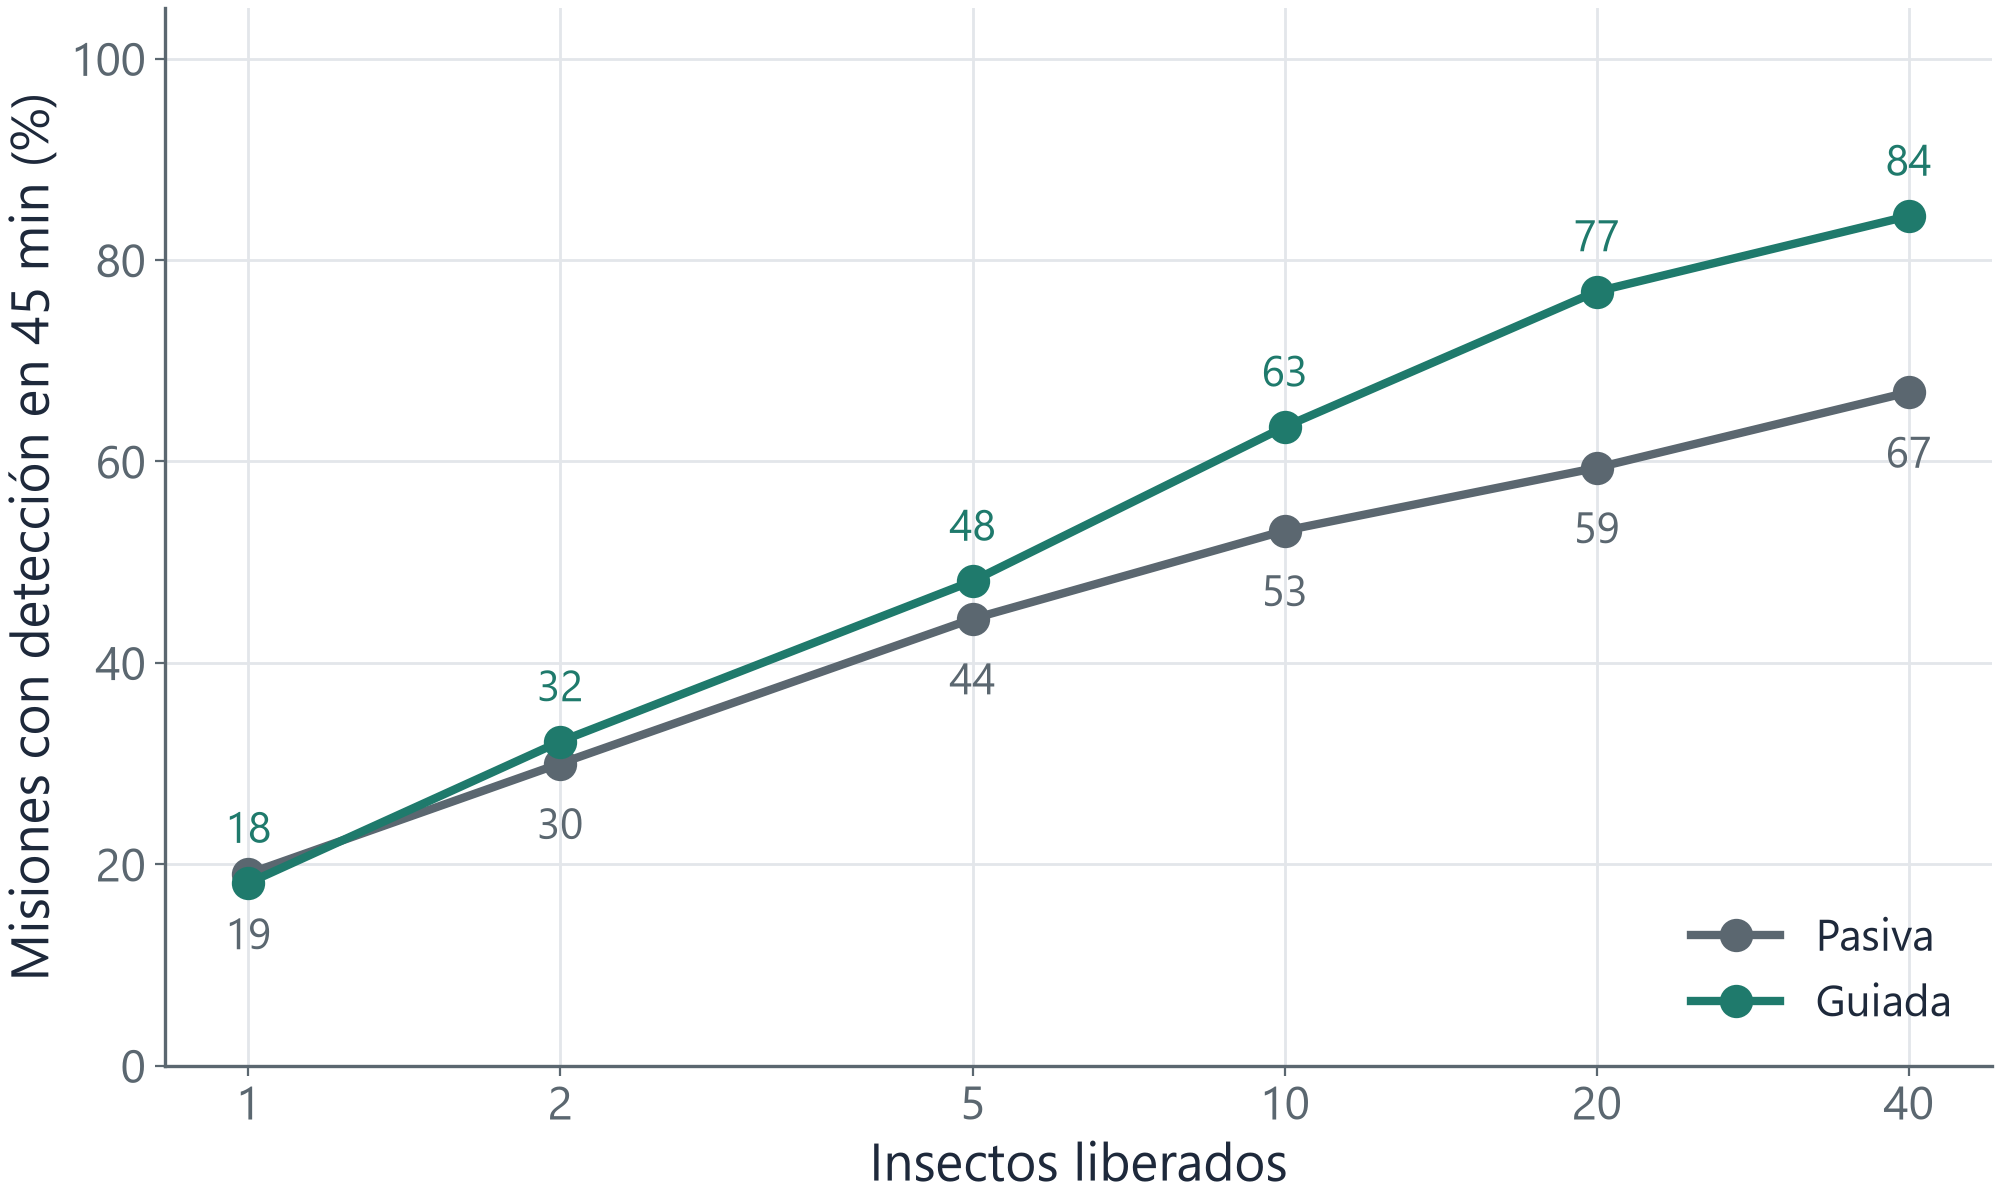
\includegraphics[width=0.62\textwidth]{figs/enjambre.png}
\caption{Detección a 45~min según el número de insectos liberados.}
\label{fig:enjambre}
\end{figure}

\begin{table}[H]
\centering\footnotesize
\caption{Detección acumulada (\%) según el número de insectos liberados.}
\label{tab:enjambre}
\rowcolors{2}{SoftGray}{white}
\begin{tabularx}{0.8\textwidth}{@{}>{\bfseries\raggedright\arraybackslash}X r r r r r r@{}}
\toprule
\rowcolor{TableHead} & \multicolumn{3}{c}{\textbf{Pasiva}} & \multicolumn{3}{c}{\textbf{Guiada}} \\
\rowcolor{TableHead} \textbf{Insectos} & 30 min & 45 min & 60 min & 30 min & 45 min & 60 min \\
\midrule
\tablaEnjambre
\bottomrule
\end{tabularx}
\end{table}

Un insecto solo casi nunca basta: guiado o no, encuentra a la persona en cerca de una de cada
cuatro misiones de una hora (\enjHoraPasivaUno{} y \enjHoraGuiadaUno~\%). La guía empieza a
notarse con cinco insectos y pesa más cuanto mayor es el enjambre: con veinte, la detección en
una hora pasa de \enjHoraPasivaVeinte{} a \enjHoraGuiadaVeinte~\%. Diez insectos guiados
(\enjHoraGuiadaDiez~\%) rinden como entre veinte y cuarenta sin guiar (\enjHoraPasivaVeinte{} y
\enjHoraPasivaCuarenta~\%). Dicho de otro modo, la política equivale a duplicar o triplicar el
enjambre sin criar ni equipar más animales.

\subsection{Sensor y habituación}

\begin{figure}[H]
\centering
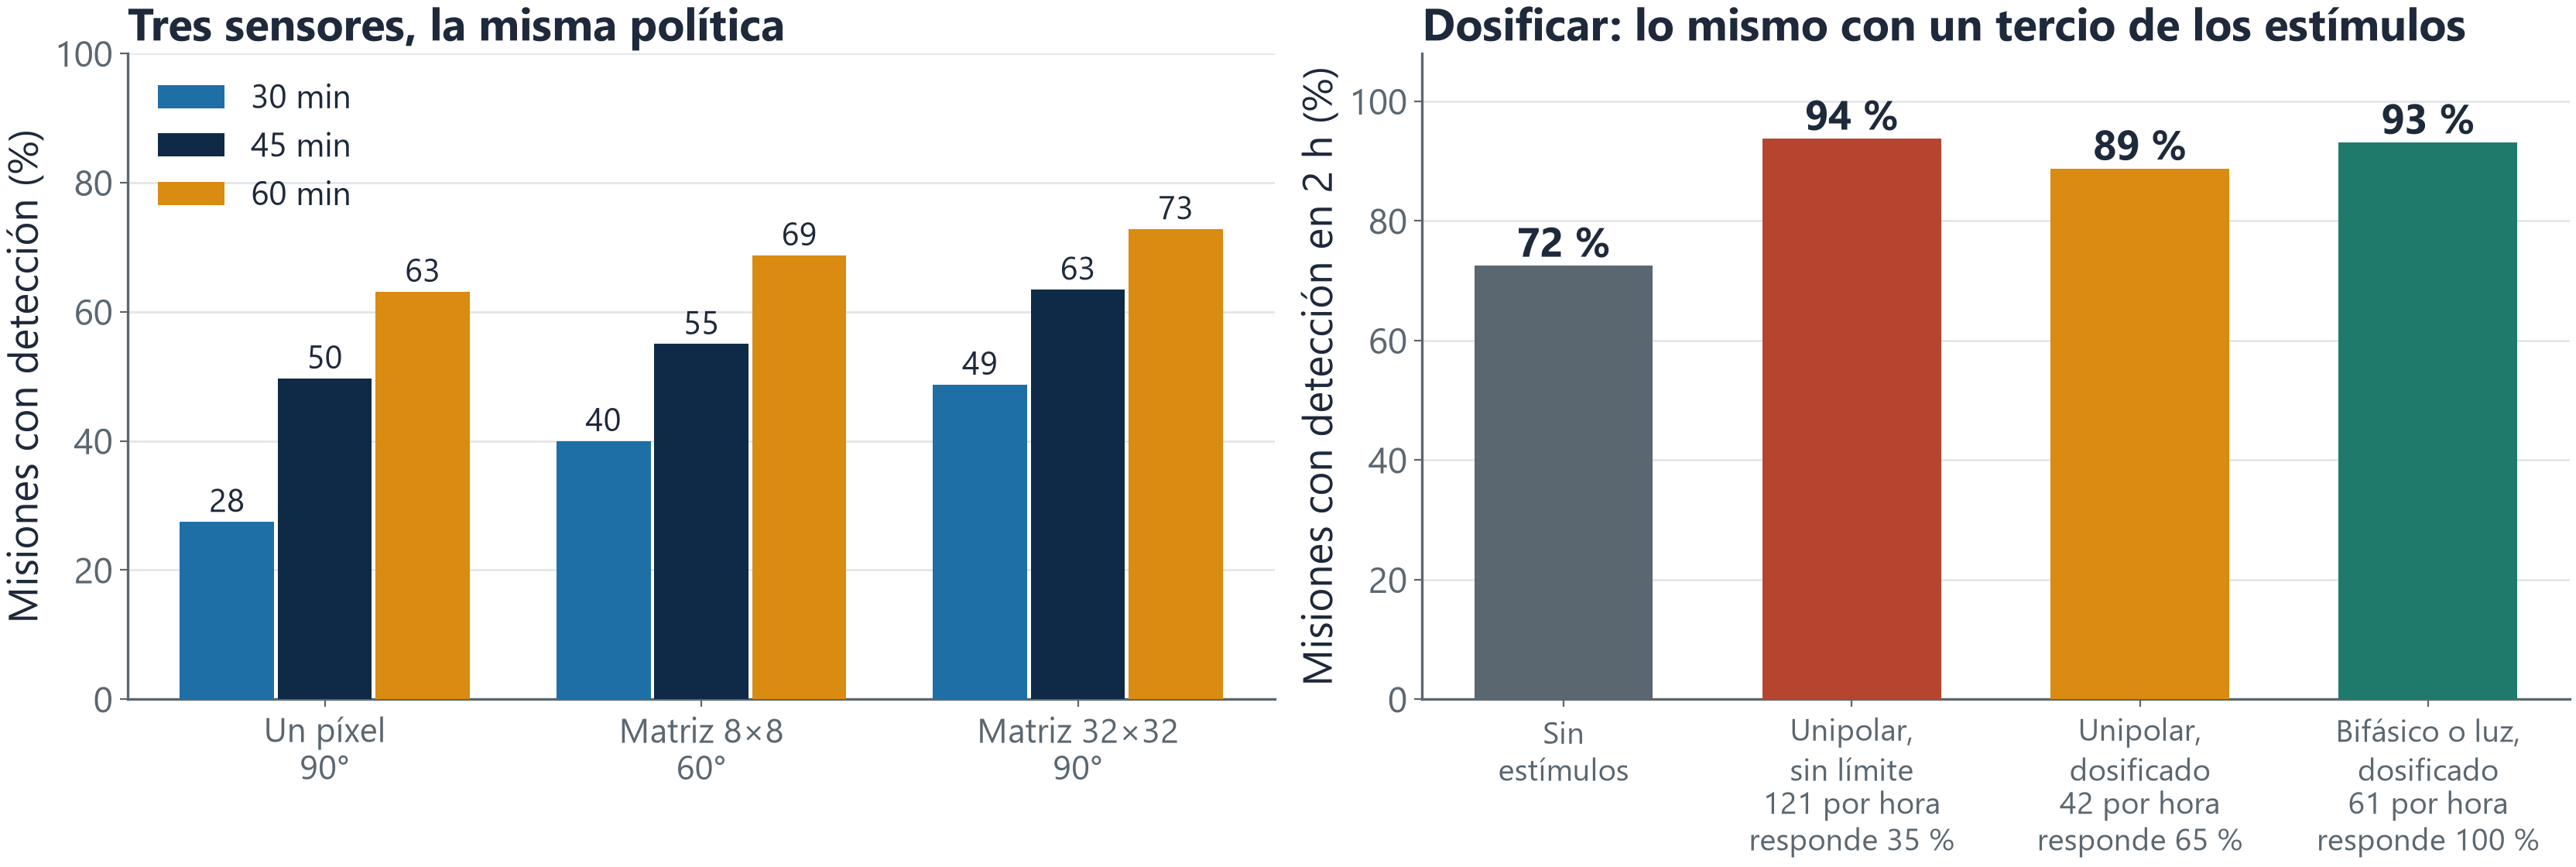
\includegraphics[width=\textwidth]{figs/sensores_habituacion.png}
\caption{Izquierda: política guiada con tres sensores. Derecha: misiones de dos horas con pulsos
unipolares, con y sin dosificación, frente a un estímulo que no habitúa.}
\label{fig:sensorhab}
\end{figure}

\textbf{El sensor cambia el resultado menos que la política.} Con la misma política guiada, la
matriz de $8\times8$ detecta en una hora en \senOchoSesenta~\% de las misiones y la de
$32\times32$ en \senTreintaDosSesenta~\%. La diferencia es mayor al principio: a los 30~min,
\senOchoTreinta{} frente a \senTreintaDosTreinta~\%. La matriz de $8\times8$, que es la que se
consigue en México, pierde pocos puntos y cuesta la mitad. El sensor de un solo punto llega a
\senPixelSesenta~\%, pero ese número lo favorece: la simulación no tiene falsas alarmas, y un
umbral de medio grado sobre el fondo las tendría.

\textbf{Dosificar no mejora la detección: la iguala con un tercio de los estímulos.} En misiones de
dos horas con pulsos unipolares, que son los que habitúan, estimular sin límite aplica
\habEstSinLimite{} estímulos por insecto y por hora y deja la respuesta en
\habRespSinLimite~\%. Con el presupuesto se aplican \habEstDosificado{} y la respuesta queda en
\habRespDosificado~\%. La detección es prácticamente la misma: \habDetSinLimite{} y
\habDetDosificado~\%, dentro del margen de muestreo. El argumento para dosificar es, entonces,
el animal y no el rendimiento: se obtiene lo mismo con la tercera parte de la carga sobre el
insecto. Con un estímulo que no habitúa, como la onda bifásica o la luz, la detección en dos
horas llega a \habDetBifasico~\%, frente a \habDetPasiva~\% sin estímulos.

\subsection{Sensibilidad a los supuestos}

Doce parámetros se movieron entre un valor bajo y uno alto, uno a la vez, en cuatro de los
colapsos (160 misiones por caso; el margen sube a unos $\pm8$ puntos). En esos cuatro colapsos
la referencia es de \sensBaseGuiada~\% de detección a 45~min para la política guiada y de
\sensBasePasiva~\% para la pasiva.

\begin{figure}[H]
\centering
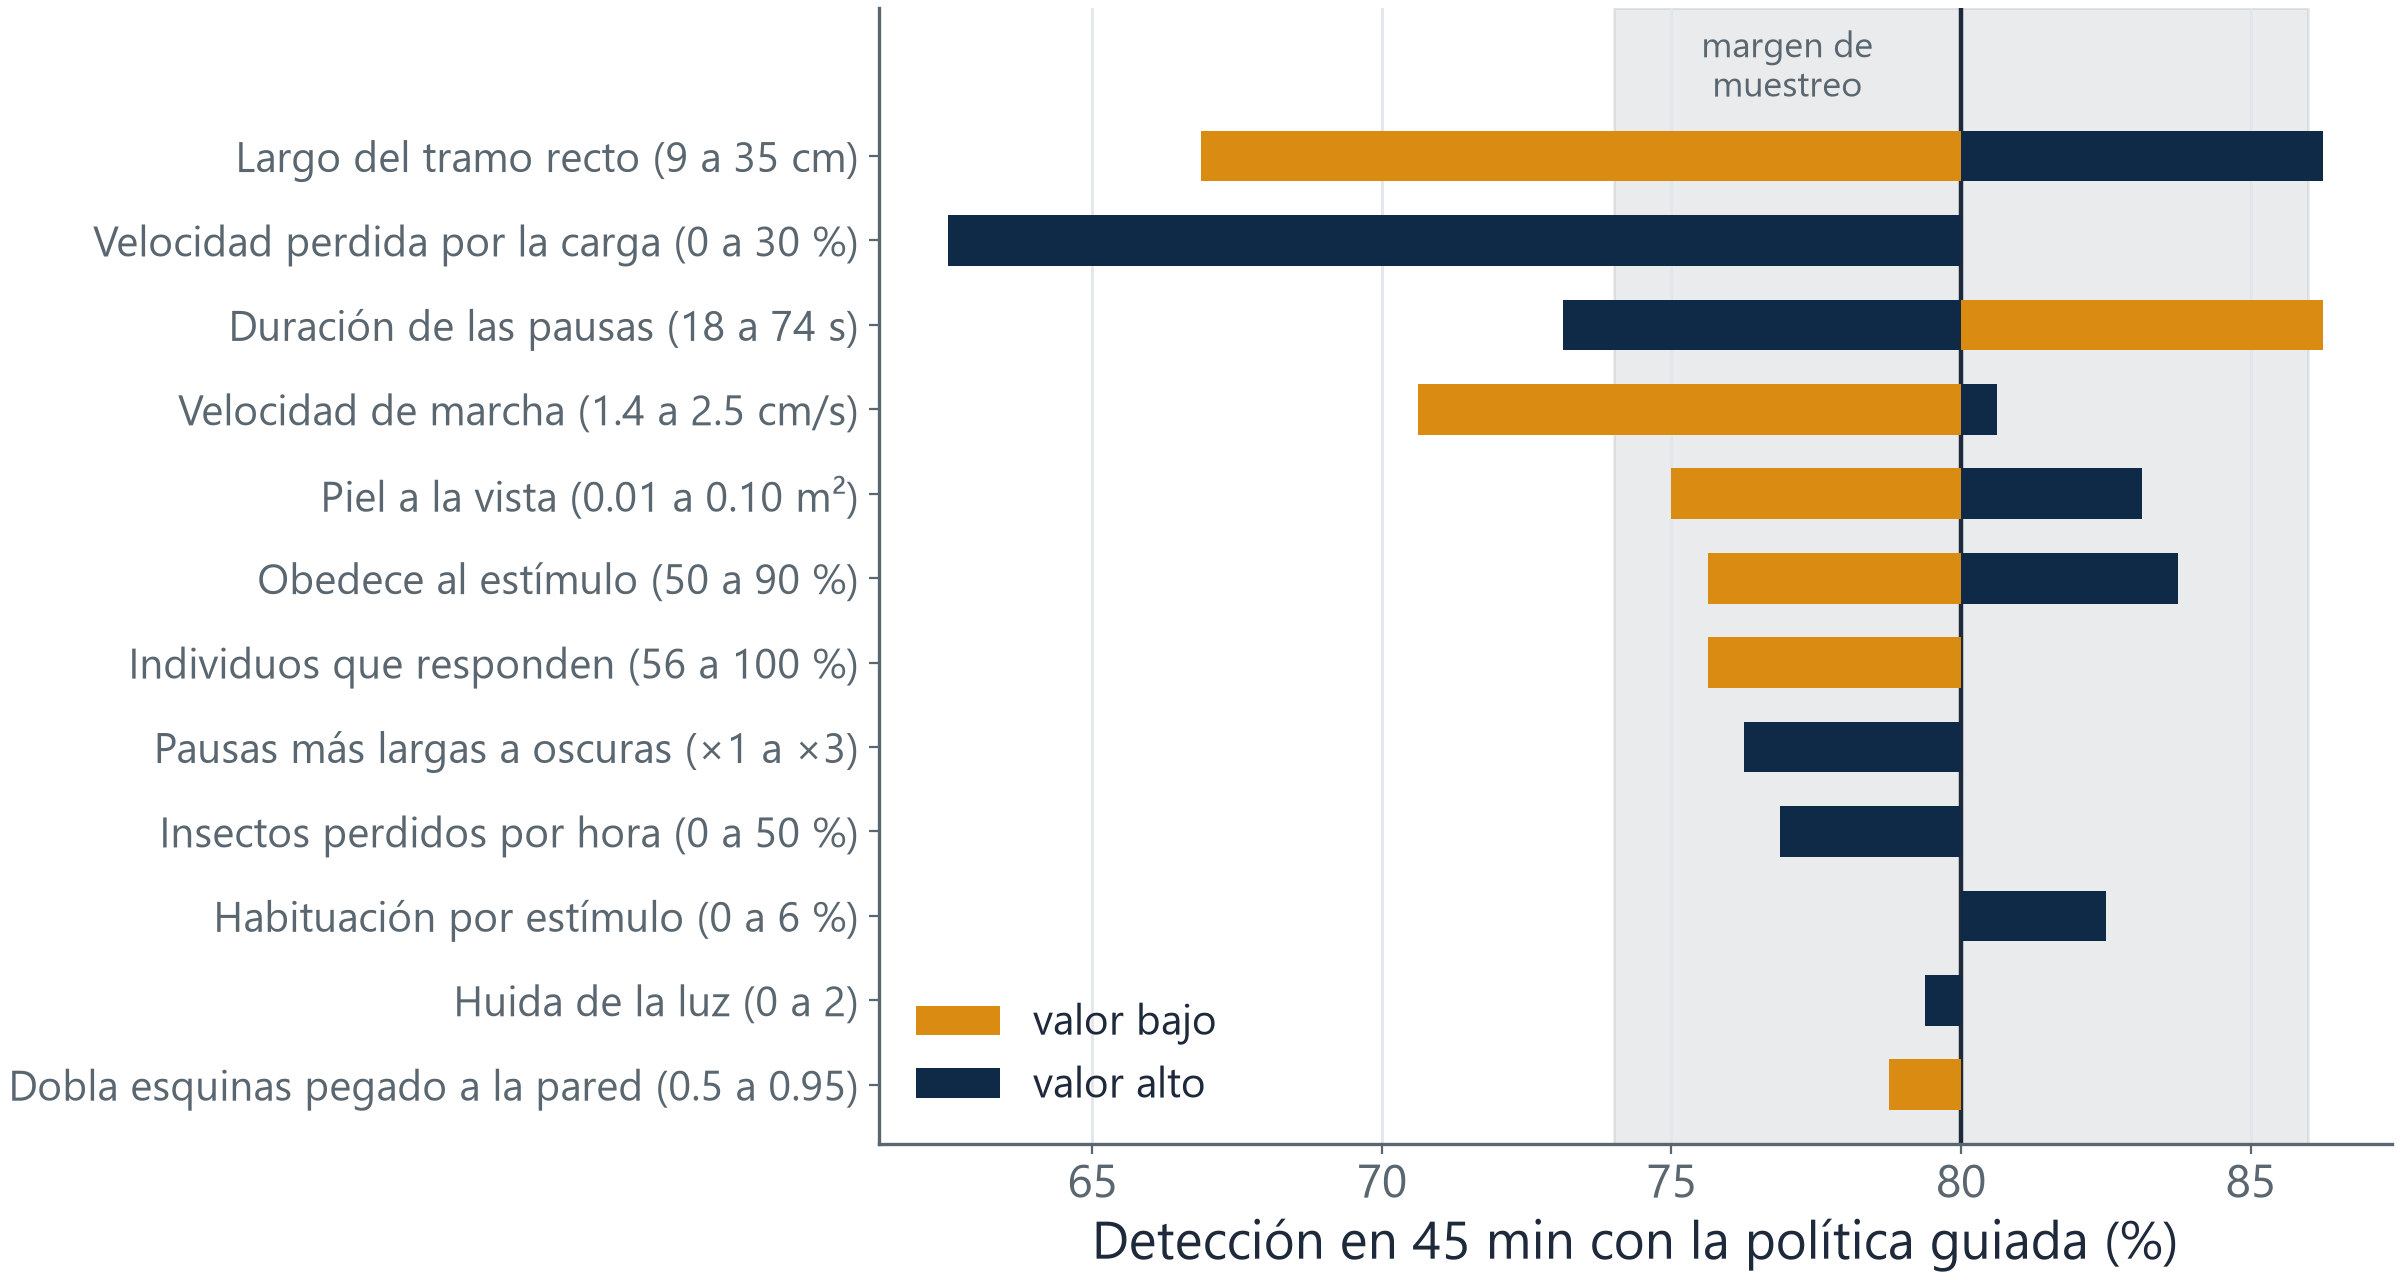
\includegraphics[width=0.86\textwidth]{figs/sensibilidad.png}
\caption{Cambio en la detección a 45~min de la política guiada al mover cada supuesto.}
\label{fig:sensibilidad}
\end{figure}

\begin{table}[H]
\centering\footnotesize
\caption{Detección a 45~min (\%) con el valor bajo y con el valor alto de cada supuesto.}
\label{tab:sensibilidad}
\rowcolors{2}{SoftGray}{white}
\begin{tabularx}{\textwidth}{@{}>{\raggedright\arraybackslash}X >{\raggedright\arraybackslash}p{3.3cm} r r r r@{}}
\toprule
\rowcolor{TableHead} & & \multicolumn{2}{c}{\textbf{Guiada}} & \multicolumn{2}{c}{\textbf{Pasiva}} \\
\rowcolor{TableHead} \textbf{Supuesto} & \textbf{Intervalo} & bajo & alto & bajo & alto \\
\midrule
\tablaSensibilidad
\bottomrule
\end{tabularx}
\end{table}

Cuatro supuestos mueven el resultado más que el margen de muestreo:
\begin{itemize}
  \item \textbf{El largo del tramo recto:} de \sensTramoBajoGuiada{} a \sensTramoAltoGuiada~\%. El insecto
        que camina tramos largos explora mejor. El dato se midió en arena abierta; entre escombro
        podría ser menor.
  \item \textbf{La velocidad que quita la carga:} de \sensCargaBajoGuiada{} a \sensCargaAltoGuiada~\% si la
        mochila le resta 30~\% de velocidad. Es el argumento numérico para la mochila ligera.
  \item \textbf{La duración de las pausas:} de \sensPausaBajoGuiada~\% con pausas cortas a
        \sensPausaAltoGuiada~\% con pausas largas.
  \item \textbf{La velocidad de marcha:} de \sensVelocidadBajoGuiada{} a \sensVelocidadAltoGuiada~\%.
\end{itemize}
Los demás (cuánto obedece, cuántos individuos responden, la habituación, la huida de la luz, la
pérdida de insectos) cambian el resultado menos que el margen de muestreo. De ahí salen dos
lecturas. La política tolera la incertidumbre sobre el estímulo, que es justo lo peor conocido. Y
lo que más importa es cuánto y qué tan rápido camina el insecto, que es lo que la carga y la
temperatura deterioran. Para la política pasiva pesa sobre todo cuánta piel queda a la vista: de
\sensAreaBajoPasiva{} a \sensAreaAltoPasiva~\%.

\subsection{Recuperar a los insectos}
\label{sec:regreso}

Una mochila que no vuelve es un animal abandonado y una pila de litio bajo el escombro. Por eso se
simuló también la segunda mitad de la misión. Tras 45~min de búsqueda guiada se da la orden de
regreso; en el boquete hay un refugio oscuro que retiene a los insectos que pasan a 30~cm de él.
Se siguió a \regInsectos{} insectos por caso durante dos horas más.

\begin{figure}[H]
\centering
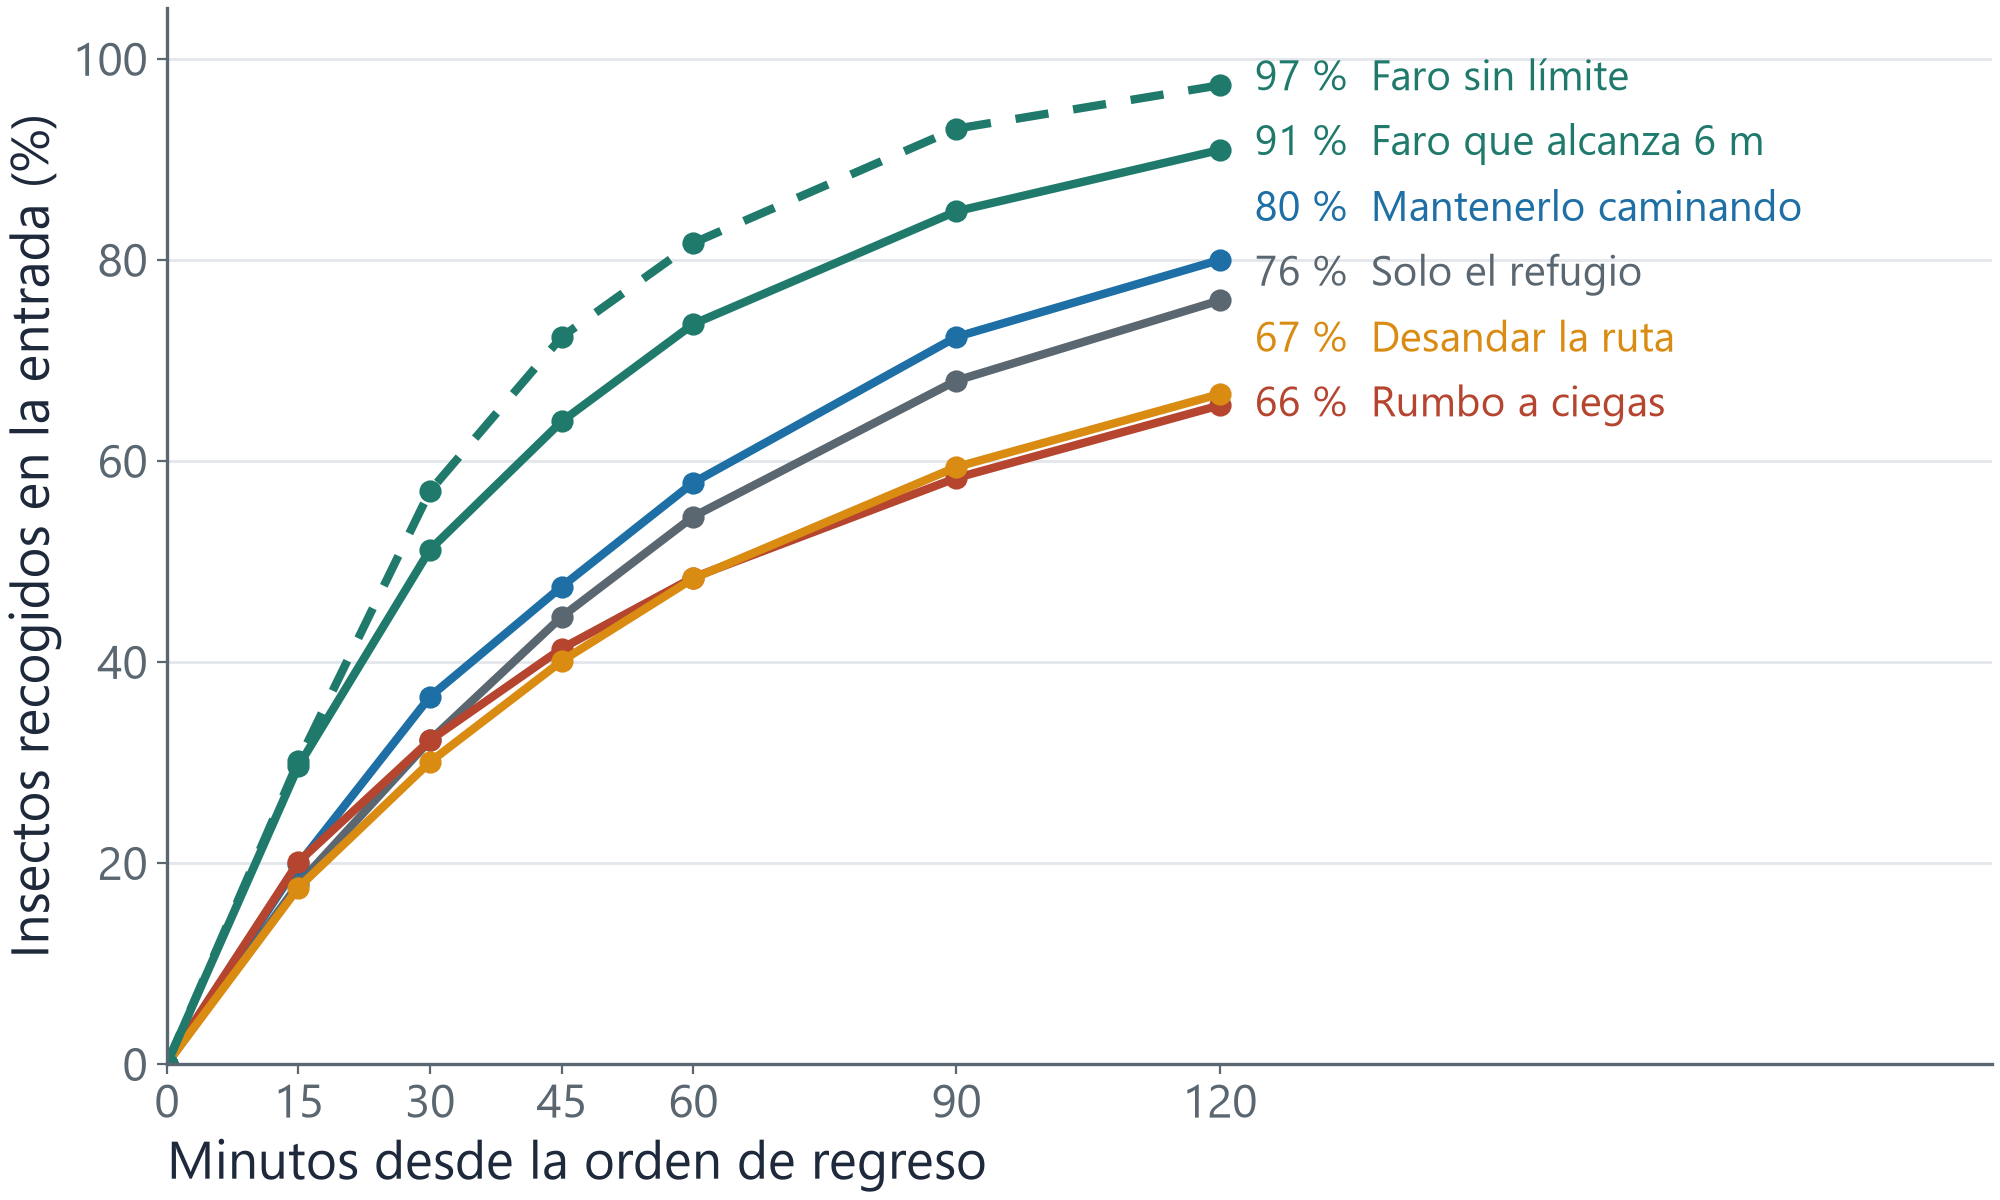
\includegraphics[width=0.74\textwidth]{figs/regreso.png}
\caption{Insectos recogidos en el refugio de la entrada, según la forma de hacerlos volver. La línea
punteada es el faro sin límite de alcance, que no es realista y marca el techo del método.}
\label{fig:regreso}
\end{figure}

\begin{table}[H]
\centering\footnotesize
\caption{Insectos recogidos (\%) después de la orden de regreso y estímulos gastados en volver.}
\label{tab:regreso}
\rowcolors{2}{SoftGray}{white}
\begin{tabularx}{0.9\textwidth}{@{}>{\raggedright\arraybackslash}X r r r r@{}}
\toprule
\rowcolor{TableHead} \textbf{Forma de regresar} & \textbf{30 min} & \textbf{60 min} & \textbf{120 min} & \textbf{Estímulos por insecto} \\
\midrule
\tablaRegreso
\bottomrule
\end{tabularx}
\end{table}

\begin{itemize}
  \item \textbf{Esperar no basta.} Con solo el refugio vuelve \regTrampaSesenta~\% en una hora y
        \regTrampaDos~\% en dos. Darle un pulso cada vez que se detiene sube poco: \regAndarDos~\%.
  \item \textbf{Guiarlo a ciegas es peor que no guiarlo.} La mochila no sabe dónde está: lo estima
        contando pasos y giros, y esa cuenta se desvía con cada metro. Ordenarle el rumbo recto a la
        entrada, o desandar la ruta guardada, recupera \regRumboDos{} y \regRutaDos~\% en dos horas.
        Es menos que el refugio solo, y cuesta \regEstRumbo{} y \regEstRuta{} estímulos por insecto.
  \item \textbf{Lo que cambia el resultado es una señal en la entrada.} Se probó un faro: una lámpara
        infrarroja en el boquete, cuya luz se cuela por los huecos, y un fotodiodo a cada lado de la
        mochila para saber de qué lado llega más. El insecto no ve esa luz; la mochila lo gira hacia
        ella con los mismos estímulos de la búsqueda. Si el faro se percibe hasta 6~m de camino,
        vuelve \regFaroSesenta~\% en una hora y \regFaroDos~\% en dos, con \regEstFaro{} estímulos
        por insecto. Con el doble de error en la medida, \regFaroRuidoDos~\%.
  \item \textbf{Ningún método los recupera a todos.} Con el faro de 6~m queda fuera
        \regFaroPerdidos~\% a las dos horas: de diez mochilas se pierde, en promedio, una por
        misión. Para esas hace falta otra cosa: que cada mochila siga emitiendo su número por
        radio, de modo que se sepa cuántas faltan y cerca de qué relevo quedaron.
\end{itemize}

El faro es un supuesto y no una medida. Nadie ha publicado cuánto se propaga una luz o un sonido
entre escombro, ni con qué error lo localiza una mochila de este tamaño. Sí existen las dos piezas
por separado: una cerca invisible que devuelve al insecto cuando sale de una zona~\cite{latif2014}
y micrófonos en la mochila para localizar una fuente de sonido~\cite{latif2016}. El modo de regreso
tampoco está en el núcleo: pide dos fotodiodos, un comparador y un estado más en la máquina.

\subsection{Qué dice y qué no dice la simulación}

\textbf{Sobre la hipótesis.} Se sostiene en parte. La política guiada aumenta la detección en una
sesión de 45 a 60~min (de \pPasivaCuarentaCinco{} a \pGuiadaCuarentaCinco~\% y de
\pPasivaSesenta{} a \pGuiadaSesenta~\%), no provoca habituación con un estímulo bifásico o de luz
y cabe en una FPGA de miligramos. Pero la mejora no es uniforme: depende del colapso, y en uno
de los ocho la política empeora el resultado. Y dosificar no mejora la detección; solo reduce la
carga sobre el insecto.

\begin{itemize}
  \item \textbf{Dice} que una política sencilla, que cabe en 181 elementos lógicos, mejora la búsqueda
        respecto de soltar a los insectos y esperar, y que lo hace con pocos estímulos.
  \item \textbf{Dice} que el número de insectos y la forma del colapso importan más que la política.
  \item \textbf{No dice} cuánto tardaría un rescate real. Los colapsos son sintéticos y planos, la marcha se
        midió en arenas iluminadas y la respuesta a la luz ultravioleta se supuso igual a la de los
        electrodos de superficie.
  \item \textbf{No dice} nada sobre falsas alarmas: en la simulación la persona es la única fuente de
        calor. Eso se medirá con el sensor real.
\end{itemize}
